\documentclass{article}
\usepackage[paperwidth=218mm,paperheight=78mm,margin=4mm,noheadfoot]{geometry}
\usepackage{amsmath,amssymb}
\usepackage{helvet}
\usepackage{tikz}
\renewcommand{\familydefault}{\sfdefault}
\usetikzlibrary{arrows.meta,backgrounds,calc,fit,positioning,shapes.geometric}

% Restrained palette adapted from the visual language of the supplied
% fast-charging transfer-optimization paper: amber data, blue optimization,
% green physical model, and one warm orange knowledge branch.
\definecolor{ink}{HTML}{263238}
\definecolor{muted}{HTML}{607D8B}
\definecolor{hair}{HTML}{B0BEC5}
\definecolor{blue}{HTML}{118ACB}
\definecolor{bluefill}{HTML}{EAF5FB}
\definecolor{orange}{HTML}{E58A3A}
\definecolor{orangefill}{HTML}{FFF2E7}
\definecolor{amber}{HTML}{E4A92B}
\definecolor{amberfill}{HTML}{FFF6D9}
\definecolor{green}{HTML}{4F8F4A}
\definecolor{greenfill}{HTML}{EDF6E9}

\tikzset{
  every node/.style={text=ink},
  block/.style={draw=hair, fill=white, rounded corners=1.6pt,
    line width=.65pt, align=center, inner xsep=4pt, inner ysep=3pt,
    font=\fontsize{9.2}{10.4}\selectfont},
  llm/.style={block, draw=orange, fill=orangefill, line width=.9pt},
  sub/.style={block, draw=blue, fill=white, minimum height=13mm,
    line width=.72pt},
  simulator/.style={block, draw=green, fill=greenfill, line width=.9pt},
  mainflow/.style={-{Latex[length=2.3mm,width=1.35mm]}, draw=ink,
    line width=.85pt},
  update/.style={-{Latex[length=2.3mm,width=1.35mm]}, draw=muted,
    line width=.8pt},
  knowledge/.style={-{Latex[length=2.2mm,width=1.3mm]}, draw=orange,
    dashed, line width=.85pt},
  label/.style={font=\fontsize{7.7}{8.6}\selectfont, text=muted,
    fill=white, inner sep=1.2pt, align=center},
  boTitle/.style={font=\fontsize{8.4}{9.4}\selectfont\bfseries,
    text=blue, fill=bluefill, inner sep=1pt}
}

\begin{document}
\thispagestyle{empty}
\noindent
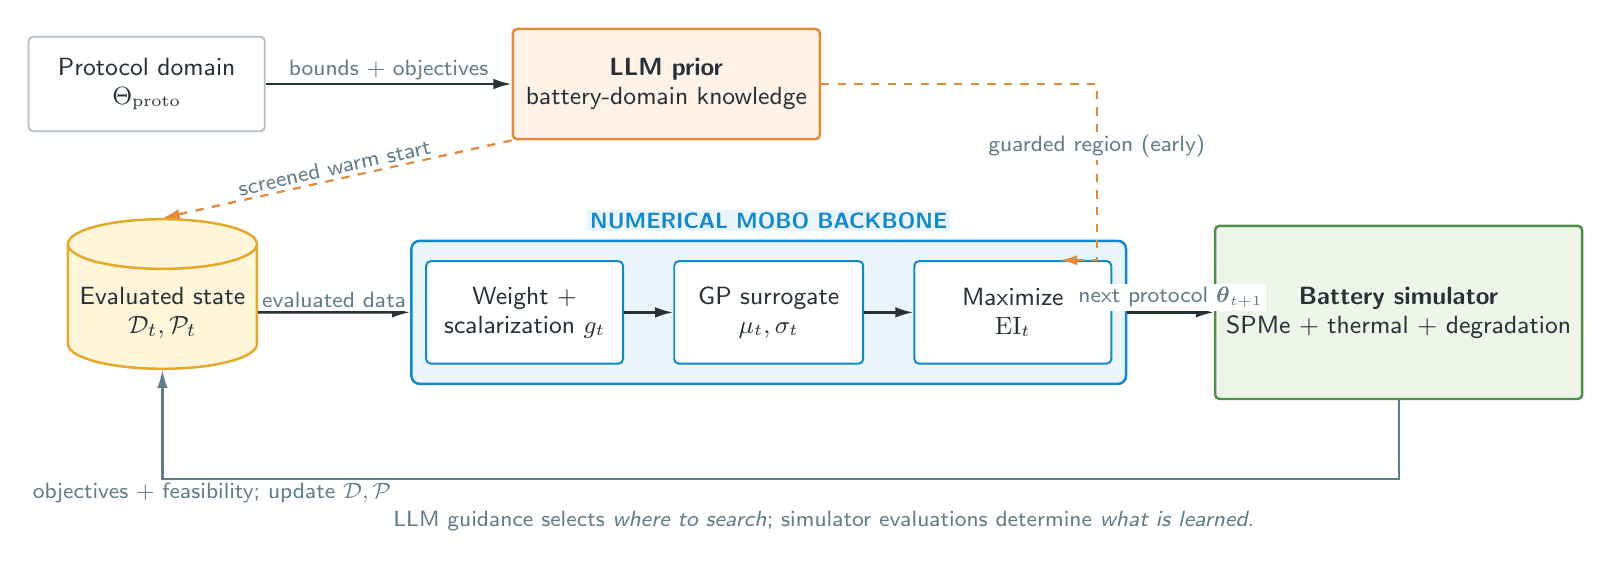
\begin{tikzpicture}[x=1mm,y=1mm]

% Domain context and LLM prior: one compact knowledge source, two bounded uses.
\node[block, minimum width=30mm, minimum height=12mm] (domain) at (22,54)
  {Protocol domain\\$\Theta_{\mathrm{proto}}$};

\node[llm, minimum width=39mm, minimum height=14mm] (llm) at (88,54)
  {\textbf{LLM prior}\\battery-domain knowledge};

\draw[mainflow] (domain) -- node[label,above]{bounds + objectives} (llm);

% Evaluated state, styled as a database icon rather than another process box.
\node[shape=cylinder, shape border rotate=90, aspect=.27,
  draw=amber, fill=amberfill, line width=.9pt,
  minimum width=24mm, minimum height=19mm,
  font=\fontsize{9.4}{10.5}\selectfont, align=center] (data) at (24,25)
  {Evaluated state\\$\mathcal D_t,\mathcal P_t$};

% Numerical backbone: algorithmic detail is nested inside one visual anchor.
\node[sub, minimum width=25mm] (scalar) at (70,25)
  {Weight +\\scalarization $g_t$};
\node[sub, minimum width=24mm] (gp) at (101,25)
  {GP surrogate\\$\mu_t,\sigma_t$};
\node[sub, minimum width=25mm] (ei) at (132,25)
  {Maximize\\$\mathrm{EI}_t$};

\draw[mainflow] (scalar) -- (gp);
\draw[mainflow] (gp) -- (ei);

\begin{scope}[on background layer]
  \node[draw=blue, fill=bluefill, rounded corners=3pt, line width=.9pt,
    fit=(scalar)(gp)(ei), inner xsep=5pt, inner ysep=7pt] (mobo) {};
\end{scope}
\node[boTitle, anchor=south] at ([yshift=1.0mm]mobo.north)
  {NUMERICAL MOBO BACKBONE};

% Physical oracle: the only component that writes objective/feasibility data.
\node[simulator, minimum width=37mm, minimum height=22mm] (sim) at (181,25)
  {\textbf{Battery simulator}\\SPMe + thermal + degradation};

% Closed-loop numerical optimization.
\draw[mainflow] (data) -- node[label,above]{evaluated data} (mobo);
\draw[mainflow] (mobo) -- node[label,above]{next protocol $\boldsymbol\theta_{t+1}$} (sim);
\draw[update] (sim.south) -- ++(0,-10) -|
  node[label,pos=.48,below]{objectives + feasibility; update $\mathcal D,\mathcal P$}
  (data.south);

% Two LLM interfaces, visually subordinate to the numerical loop.
\draw[knowledge] (llm.south west) --
  node[label,sloped,above]{screened warm start} (data.north);
\draw[knowledge] (llm.east) -- ++(35,0) |-
  node[label,pos=.22,above]{guarded region (early)}
  ([xshift=6mm]ei.north);

% One quiet invariant instead of a boxed warning or legend.
\node[font=\fontsize{8.0}{9.0}\selectfont, text=muted, align=center]
  at (108,-1.5)
  {LLM guidance selects \emph{where to search}; simulator evaluations determine \emph{what is learned}.};

\end{tikzpicture}
\end{document}
